\documentclass[tikz,border=3.14mm]{standalone}
\usetikzlibrary{positioning,calc}

\begin{document}
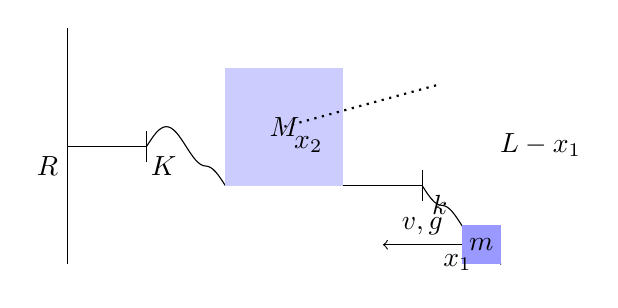
\begin{tikzpicture}
    % Draw the vertical wall
    \draw (-1,0) -- (-1,3);
    
    % Draw the left spring
    \draw (-1,1.5) -- (0,1.5);
    \draw (0,1.3) -- (0,1.7); % Spring line thickening
    \draw (0,1.5) sin (0.25,1.75) cos (0.5,1.5);
    \draw (0.5,1.5) sin (0.75,1.25) cos (1,1);
    \node at (0.5,1.5) [below left] {$K$};
    \node at (-1,1.5) [below left] {$R$};
    
    % Draw the big mass
    \fill[blue!20] (1,1) rectangle (2.5,2.5);
    \node at (1.75,1.75) {$M$};
    
    % Draw the right spring
    \draw (2.5,1) -- (3.5,1);
    \draw (3.5,0.8) -- (3.5,1.2); % Spring line thickening
    \draw (3.5,1) sin (3.75,0.75) cos (4,0.5);
    \draw (4,0.5) sin (4.25,0.25) cos (4.5,0);
    \node at (3.5,1) [below right] {$k$};
    
    % Draw the small mass
    \fill[blue!40] (4,0) rectangle (4.5,0.5);
    \node at (4.25,0.25) {$m$};
    
    % Define distances
    \coordinate (massM) at (1.75,1.75); % Position of big mass
    \coordinate (massm) at (4.25,0.25); % Position of small mass
    
    % Draw the distance arrow and label
    \draw[dotted,thick] (massM) -- ($(massm)!(massM)!(3.5,3)$); % dotted line from big mass towards upper right
    \draw[->] (4,0.25) -- ++(-1,0) node[midway,above] {$v, g$}; % arrow from small mass to left
    
    % Label the distance
    \node at ($(massm)!(massM)!(4.5,3)$) [right] {$L-x_1$};
    \node at (massM) [below right] {$x_2$};
    \node at (massm) [below left] {$x_1$};
\end{tikzpicture}
\end{document}